\documentclass[12pt, twoside]{article}
% \documentclass[12pt, twoside]{article}
\usepackage[letterpaper, margin=1in, headsep=0.2in]{geometry}
\setlength{\headheight}{0.6in}
%\usepackage[english]{babel}
\usepackage[utf8]{inputenc}
\usepackage{microtype}
\usepackage{amsmath}
\usepackage{amssymb}
%\usepackage{amsfonts}
\usepackage[nomessages]{fp} %\FPeval{\var-name}{2*sin(pi/6)}
\usepackage{siunitx} %units in math. eg 20\milli\meter
\usepackage{yhmath} % for arcs, overparenth command
\usepackage{tikz} %graphics
\usetikzlibrary{quotes, angles, arrows, arrows.meta}
\usepackage{graphicx} %consider setting \graphicspath{{images/}}
\usepackage{parskip} %no paragraph indent
\usepackage{enumitem}
\usepackage{multicol}
\usepackage{venndiagram}

\usepackage{fancyhdr}
\pagestyle{fancy}
\fancyhf{}
\renewcommand{\headrulewidth}{0pt} % disable the underline of the header
\raggedbottom
\hfuzz=2mm %suppresses overfull box warnings

\usepackage{hyperref}
\usepackage{float}

\usepackage{pgfplots}
\pgfplotsset{width=9cm,compat=1.9}

\fancyhead[LE]{\thepage}
\fancyhead[RO]{\thepage \\ Name: \hspace{4cm} \,\\}
\fancyhead[LO]{BECA / Dr. Huson / Modeling \& Mathematics Applications\\* Quantifying Uncertainty: Probability \\* 29 February 2024}

\begin{document}
\begin{enumerate}
\subsubsection*{1.22 PreExam: Probability, Venn diagrams}
\item Given: \\*
    $U = \{\text{the letters in the alphabet}\}$ \qquad
    $A = \{t, i, m, e, s\}$ \qquad
    $B = \{m, i, n, u, s\}$
    \begin{enumerate}[itemsep=1cm]
        \item List the members of $A \cup B$. \hfill [1 mark]
        \item List the elements of $A \cap B$. \hfill [1 mark]
        \item A letter is selected at random. What is the probability that it is a member of both sets, ($A \cap B$)? \hfill [1 mark]
    \end{enumerate} \vspace{1.5cm}

\item Events $A$ and $B$ are independent with $\mathrm P(A)=0.3$, $\mathrm P(B)=0.5$. Find each probability.
    \begin{enumerate}[itemsep=0.8cm]
        \item $\mathrm P(A \cap B)$ \hfill [2 mark]
        \item $\mathrm P(A \cup B)$ \hfill [2 mark]
        \item $\mathrm P(B' \cap A)$ \hfill [2 mark]
        \item $\mathrm P(A | B)$ \hfill [2 mark]
        \item Mark the Venn diagram with the probabilities for each area. \hfill [2 marks]
    \end{enumerate}
    \begin{center}
        \begin{venndiagram2sets}[tikzoptions={scale=1.75}]
        \end{venndiagram2sets}U
    \end{center}


\newpage
\item The universal set $U$ is defined as the set of positive integers less than 13.
    \begin{enumerate}[itemsep=1.2cm]
        \item Subset is defined as $A =$ \{multiples of three\}. List its elements.  \hfill [1 mark] 
        \item Subset  $B =$ \{perfect squares\}. List the members of set $B$.  \hfill [1 mark]
        \item List the members of $(A \cup B)'$.  \hfill [1 mark]
        \item Place the elements of $U$ in the appropriate regions in the Venn diagram. \hfill [2 marks]
        \begin{center}
            \begin{venndiagram2sets}[tikzoptions={scale=2}]
            \end{venndiagram2sets}U
        \end{center}
        \item If an element is selected at random, what is the probability that it is a member of both sets, ($A \cap B$)? \hfill [1 mark]
        \item If a member of set $B$ is selected at random, what is the probability that it is also a member of set $A$, i.e. the conditional probability ($A | B$)? \hfill [2 mark]
    \end{enumerate}

\newpage
\item A jar contains 30 marbles, 12 of which are red, 8 are blue, and 10 are green.
    \begin{enumerate}[itemsep=1.5cm]
        \item A marble is selected at random. Find the probability it is red. \hfill [1 mark]
        \item The marble is replaced and a second marble is selected. Given that the second marble is not red, find the probability it is blue. \hfill [1 mark]
        \item The marbles are returned to the jar and two marbles are selected at random. Find the probability that both are green. \hfill [2 mark]
    \end{enumerate} \vspace{1.5cm}

\item Draw a tree diagram to represent the taxi cab problem in the textbook. First, there are two cab companies, 85\% are black and the rest are yellow. Then, the witness identifies the color of the cab correctly 80\% of the time. \hfill [3 marks]
\begin{enumerate}
    \item Label the branches with the probabilities. \hfill [1 marks]
    \item Calculate the probabilities of each four outcomes. \hfill [2 marks]
    \item Given that the witness identified the cab as yellow, find the probability that it was black, i.e. that she was wrong. \hfill [3 marks]
\end{enumerate}

\newpage
\item \; \\
    \includegraphics[scale=0.5]{../graphics/problem15-p374.png} \vspace{2cm}

\item The events $A$ and $B$ are mutually exclusive with $\mathrm P(A)=0.30$ and $\mathrm P(B)=0.15$.
    \begin{enumerate}[itemsep=1.5cm]
        \item Write down $\mathrm P(A \cap B)$. \hfill [1 mark]
        \item Write down $\mathrm P(A \cup B)$. \hfill [1 mark]
    \end{enumerate}

\newpage
\item Given events $A$ and $B$ with $\mathrm P(A)=0.5$, $\mathrm P(B)=0.6$, $\mathrm P(A \cap B)=0.35$.
    \begin{enumerate}
        \item Completely mark the Venn diagram with probabilities for each area. \hfill [2 marks]
        \begin{center}
            \begin{venndiagram2sets}[tikzoptions={scale=1.5}]
            \end{venndiagram2sets}
        \end{center}
        \item Find $\mathrm P(A \cup B)$. \hfill [2 marks] \vspace{1.5cm}
        \item State whether events $A$ and $B$ are independent. Justify your answer. \hfill [3 marks] \vspace{2.5cm}
    \end{enumerate}

\item For each Venn diagram, write an expression representing the shaded area. \hfill [5 marks] 
    \begin{multicols*}{2}
    \begin{enumerate}
        \item 
        \begin{venndiagram2sets}
            \fillACapB
            %\fillB
        \end{venndiagram2sets}
        \item %\\*[15pt]
            \begin{venndiagram2sets}
            \fillANotB
            \end{venndiagram2sets}
        \item %\\*[15pt]
        \begin{venndiagram2sets}
            \fillA
            \fillB
        \end{venndiagram2sets}
        \item %\*[15pt]
            \begin{venndiagram3sets}
            \fillANotC
            \fillBNotC
            \end{venndiagram3sets}
    \end{enumerate}
    \end{multicols*}

\newpage
\item There are 60 students enrolled in the following courses:
    \begin{itemize}
        \item 28 take Archery
        \item 30 take Biology
        \item 22 take Calculus
        \item 8 take Archery and Biology
        \item 7 take Archery and Calculus
        \item 10 take Biology and Calculus
        \item 5 take all three classes
    \end{itemize}
Complete the Venn diagram below with the number of students in each region to represent the situation. \hfill [4 marks] 
    \begin{center}
        \begin{venndiagram3sets}[tikzoptions={scale=2.5}]
        \end{venndiagram3sets}U
    \end{center}

\newpage
\item For each Venn diagram, write an expression representing the shaded area.
\begin{enumerate}
    \item For example, for this diagram \\*
    %\\*
    \begin{venndiagram2sets}
        \fillANotB
        %\fillB
    \end{venndiagram2sets}
    Expression: $A \cap B'$\\*
    \item %\\*[15pt]
    \begin{venndiagram2sets}
        \fillNotB
    \end{venndiagram2sets}
    Expression: %\\*
    \item %\\*[15pt]
    \begin{venndiagram2sets}
    \fillBNotA
    \end{venndiagram2sets}
    Expression: %\\*
    \item %\*[15pt]
    \begin{venndiagram3sets}
    \fillB
    \fillCCapA
    \end{venndiagram3sets}
    Expression: %\\*
\end{enumerate}

\newpage
\item Given: \\*
\qquad $U = \{\text{the letters in the alphabet}\}$\\*
\qquad $A = \{a, b, c, d, e, f, g, h, i, j\}$
\qquad $B = \{h, i, j, k, l, m, n, o, p, q\}$
\begin{enumerate}
    \item What is $A \cap B$?\\*[20pt]
    \item What is $(A \cup B)'$?\\*[20pt]
\end{enumerate}

\newpage
\item For each Venn diagram, shade the area representing the expression. Use pencil.
    \begin{enumerate}
        \item $A \cup B$ \hspace{2cm}
            \begin{venndiagram2sets}
                %\fillANotB
                %\fillB
            \end{venndiagram2sets} \hfill [2 marks]
        \item $A' \cap B$ \hspace{2cm}
            \begin{venndiagram2sets}
            \end{venndiagram2sets} \hfill [2 marks]
        \item $(A \cap B) \cup C$ \hspace{1cm}
            \begin{venndiagram3sets}
            \end{venndiagram3sets} \hfill [2 marks]
    \end{enumerate}

\newpage
    \item Forty IB high school students range in age from 15 to 18 years old. The following table shows the frequencies of each age.
        \begin{center}
            \begin{tabular}{|l|r|r|r|r|}
                \hline
                Age (years) & 15 & 16 & 17 & 18\\ 
                \hline 
                Frequency & 5 & $k$ & 15 & 7\\ 
                \hline 
                \end{tabular}      
        \end{center}
        \begin{enumerate}[itemsep=0.8cm]
            \item Calculate the value of $k$. \hfill [1 mark]
            \item Write down the mode. \hfill [1 mark]
            \item Find the value of the range. \hfill [1 marks]
            \item Find the median. \hfill [1 marks]
            \item Find the mean. \hfill [2 marks]
            \item Find the standard deviation. \hfill [2 marks]
        \end{enumerate} \vspace{0.5cm}

    \item A runner records her pace in terms of distance run ($d$) in miles over time ($t$) in minutes during a 4.5 mile run. She models her pace with a linear regression equation $d=at+b$.
        \begin{center}
        \begin{tabular}{|l|c|c|c|c|c|}
            \hline
            minutes ($t$) & 0 & 8 & 15 & 22 & 30 \\ 
            \hline 
            miles ($d$) & 0 & 1.8 & 2.7 & 3.7 & 4.5 \\ 
            \hline 
            \end{tabular}
        \end{center}
        \begin{enumerate}[itemsep=3.5cm]
            \item Find the values of $a$, $b$, and the correlation $r$. \hfill [3 marks]
            \item Explain what the value of $a$ represents in the context of the situation. \hfill [2 marks]
        \end{enumerate}

\newpage
    \item The following diagram shows triangle $ABC$ (not drawn to scale).
    \begin{center}
    \begin{tikzpicture}[scale=1.4, rotate=-15]
        \draw [-, thick] (54:3) node[above right]{$C$}--
        (0,0) node[left]{$A$}--
        (4.5,0) node[right]{$B$}--cycle;
        \node at (0.3, 0.2)[right]{$53^\circ$};
        \node at (4, 0.2)[above left]{$41^\circ$};
        \node at (3.3, 1.7)[below]{$12$};
    \end{tikzpicture}
    \end{center} 
    $BC=12$, $C\hat{A}B=53^\circ$, and $A\hat{B}C=41^\circ$
    \begin{enumerate}
        \item Find the measure of $A\hat{C}B$. \hfill [1 mark] \vspace{3cm}
        \item Find $AC$. \hfill [3 marks] \vspace{5cm}
        \item Find the area of triangle $ABC$. \hfill [3 marks] \vspace{5cm}
    \end{enumerate}
    
\newpage
    \item The histogram below shows the weight $w$ in kilograms for 70 professional football players.

    \begin{center}
        \begin{tikzpicture}
        \begin{axis}[
        xlabel=Weight (kilograms),
        ylabel=Frequency,
        ybar interval=1,
        xmin=60, xmax=195,
        ymin=0, ymax=24,
        xtick={70,90,110,130,150,170,190},
        ytick={0,2,4,6,8,10,12,14,16,18,20,22},
        axis lines = left,
        ymajorgrids=true,
        axis x discontinuity=crunch,
        ]
        \addplot+ [color=black, fill=lightgray]
        coordinates {(80,5) (100,14)
            (120,21) (140,17) 
            (160,13) 
            (180,3)}; %Last pair does not show
        \end{axis}
        \end{tikzpicture}
    \end{center}

    The following is the frequency table for the distribution of $w$. \\[0.25cm]
        \begin{tabular}{|l|c|c|c|c|c|}
        \hline
        HR ($x$) & $70 \leq x < 90$ & $90 \leq x < 110$ & $110 \leq x < 130$ & $130 \leq x < 150$ & $150 \leq x < 170$ \\ 
        \hline 
        Freq & 5 & 14 & 21 & $p$ & 13  \\ 
        \hline 
        \end{tabular}
        \begin{enumerate}
        \item Write down the value of $p$. \hfill [1 mark] \vspace{0.8cm}
        \item Write down the modal class. \hfill [2 marks] \vspace{0.8cm}
        \item A player is selected at random. Find the probability that the athlete weighs less than 110 kilograms. \hfill [2 marks] \vspace{1cm}
        \item Write down the mid-interval value for the class $110 \leq x < 130$. \hfill [1 mark] \vspace{0.8cm}
        \item Hence find an estimate for the
        \begin{enumerate}
            \item mean; \hfill [2 marks] \vspace{0.8cm}
            \item standard deviation. \hfill [2 marks] 
        \end{enumerate}
        \end{enumerate}

\newpage
\item A survey question has three possible responses: $A$, $B$, and $C$. Among 100 surveys, the frequency of the answers collected were as follows: $n(A)=10, n(B)=35, \text{ and } n(C)=55$.
\begin{enumerate}
    \item If a survey is selected at random, what this the probability the response was $B$ or $C$?  \vspace{1cm}
    \item What is the probability a survey selected at random was an answer other than $B$ or $C$?  \vspace{1cm}
\end{enumerate}

\end{enumerate}
\end{document}